\scanpage{28}
\mspage{9}
is equivalent to the \deleted{identical} \deleted{corresponding} \inserted{analogous} equation in $\widetilde\alpha$
\[
(26)\qquad\widetilde\alpha\rho^{-1}(\widetilde\alpha)\rho^{-2}(\widetilde\alpha)=1,
\qquad\boxed{(27)\quad\widetilde\alpha=\eta^{-1}l_0^\gamma\varepsilon_0(\eta)}
\]
\deleted{$\unsure{\varepsilon}$}
Let us now consider the groupoid \inserted{$\overline{\underline{\mathrm{III}}}_J$} induced by the preceding groupoid \inserted{$\overline{\underline{\mathrm{II}}}_J$} on the set of the three vertices $Q_i$, it is also the groupoid generated by the graph with three vertices $Q_i$ $(i\in J)$ and six oriented arcs $\widetilde a_i^\omega$ and their opposites, with only the relations $(16)$ (set of 6 relations stable under $G_J$, and in fact reducing to two effective relations\ldots).
\figure{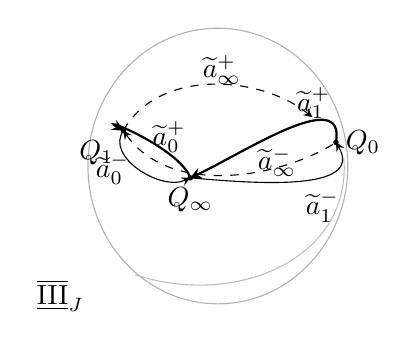
\begin{tikzpicture}[x=1cm,y=1cm,>=stealth]
\draw[gray!60] (0,.1) ellipse (1.65 and 1.75);
\draw[gray!50] (-1.05,-1.28) .. controls (.2,-1.7) and (1.7,-1.1) .. (1.6,.2);
\coordinate (A) at (-1.2,.55);\coordinate (B) at (-.35,-.05);\coordinate (C) at (1.5,.4);
\foreach \p in {A,B,C}{\fill(\p) circle(.035);}
\draw[->,thick] (B) to[out=110,in=150] node[right] {$\widetilde a_0^+$} (A);
\draw[->] (A) to[out=235,in=205] node[left] {$\widetilde a_0^-$} (B);
\draw[->,thick] (C) to[out=80,in=25] node[above right] {$\widetilde a_1^+$} (B);
\draw[->] (B) to[out=-5,in=300] node[below right] {$\widetilde a_1^-$} (C);
\draw[->,dashed] (A) .. controls (-.75,1.35) and (.55,1.25) .. (1.2,.72);
\node at(.05,1.32){$\widetilde a_\infty^+$};
\draw[<-,dashed] (A) .. controls (-.6,-.3) and (.8,-.05) .. (C);
\node at(.75,.15){$\widetilde a_\infty^-$};
\node[below left] at(A){$Q_1$};\node[below] at(B){$Q_\infty$};\node[right] at(C){$Q_0$};
\node at(-2,-1.55){$\overline{\underline{\mathrm{III}}}_J$};
\end{tikzpicture}}
The group $\{1,\tau\}$ acts there on the graph with relations, by
\[
(27)\qquad\tau Q_i=Q_i,\quad\tau\widetilde a_i^\omega=(\widetilde a_i^{\omega'})^{-1}
\]
Giving an \deleted{automorphism} \inserted{endomorphism} of the groupoid $\overline{\underline{\mathrm{III}}}_J$, fixing the vertices and commuting with $G_J$, is equivalent to giving an $\widetilde\alpha\in\widehat\Pi_{0,3}$, \deleted{$\unsure{\in\widehat{\mathbb Z}}$}, satisfying \deleted{\unsure{the equation rel.}} $(26)$. We will have, on introducing
\[
(28)\qquad\widetilde\lambda_i^\omega=\widetilde a_i^{\omega'}\widetilde a_i^\omega\in\deleted{\unsure{Q_{\omega'i}}}\inserted{\pi(Q_{\omega'i})}
\]
(compare with the definition in the groupoid $\overline{\underline{\mathrm{II}}}_J$ ! $\lambda_i^\omega=a_i^{\omega'}a_i^\omega$)
\diagram{\begin{tikzcd}[ampersand replacement=\&,column sep=small]
Q_{\omega i}\arrow[rrr,bend right=45,"\widetilde a_i^{\omega'}"']\&R_i^{\omega'}\arrow[l,dashed,no head]\arrow[r,dashed,bend right=40]\&R_i^\omega\arrow[l,dashed,bend right=40,"a_i^\omega"']\arrow[r,dashed,no head]\&Q_{\omega'i}\arrow[lll,bend right=45,"\widetilde a_i^{\omega\deleted{\unsure{'}}}"']
\end{tikzcd}}
\margin{\deleted{it would seem reasonable to change the notation $\widetilde a_i^\omega$ becoming $\widetilde a_i^{\omega'}$.}\quad $*$ \unsure{hold|obtain}, \unsure{a definition of the} $\psi_i^\alpha$ \unsure{which} \unsure{gives} in $(29)$ \unsure{thus the}. cf. see below}
\[
(29)\qquad u(\widetilde\lambda_i^\omega)=\overset{*}{\psi_{\omega'i}^{\omega'}}(\widetilde\alpha\varepsilon_0(\widetilde\alpha))\widetilde\lambda_i^\omega
=\psi_{\omega'i}^{\omega'}(\widetilde\alpha\varepsilon_0(\widetilde\alpha)l_0)
\]
In the case where $\widetilde\alpha$ comes from $\eta,\gamma$ by $(27)$, we will have
\[
(30)\qquad\widetilde\alpha\varepsilon_0(\widetilde\alpha)l_0=\eta^{-1}l_0^p\eta\qquad(p=2\gamma+1)\ ;
\]
\margin{27}
